\begin{fullwidth}

\vspace{10 mm}
\begin{problem}
Four people begin on the same side of a bridge. You must send them across to the other side in the fastest time possible. It is night. There is one flashlight. A maximum of two people can cross at a time. Any party who crosses, either one or two people, must have the flashlight to see. The flashlight must be walked back and forth, it cannot be thrown, etc. Each person walks at a different speed. A pair must walk together at the rate of the slower person's pace, based on this information: Person $1$ takes $t_1 = 1$ minutes to cross, and the other persons take $t_2 = 2$ minutes, $t_3 = 5$ minutes, and $t_4 = 10$ minutes to cross, respectively. 
\end{problem}

\end{fullwidth}

G\"unter Rote\footnote{\bibentry{Rote02}} gives a very elegant solution to this puzzle.

\subsection{How many ways are there to let $n$ people cross the bridge under the rules of the original puzzle ?}

There are $\binom{n}{2}$ ways to send the first pair over to the other side, there are 2 ways to send the flashlight back with somebody from that side.  Now there are $\binom{n -1}{2}$ ways to send the next pair over to the other side from the remaining $n - 1$ people on this side and then there are 3 ways to send the flashlight back with somebody from that side etc.
 
Using the basic product counting principle from combinatorics we get the number of ways $P$ to let $n$ people cross the bridge

\begin{equation}
\begin{aligned}
P & = \binom{n}{2} 2 \binom{n - 1}{2} 3 \binom{n - 2}{2} 4 \dots (n - 1) \binom{2}{2} \\
    & = (n - 1) ! \prod_{k = 0}^{n - 2} \binom{n - k}{2}
\end{aligned}
\label{mainFormula}
\end{equation}

Taking the product from (\ref{mainFormula}) and using the definition of a binomial coefficient we get:

\begin{equation}
 \prod_{k = 0}^{n - 2} \binom{n - k}{2} =  \prod_{k = 0}^{n - 2} \frac{(n - k) !}{2 ! (n - k - 2)!}
 \label{productPart}
\end{equation}

\noindent With:

\begin{equation}
\begin{aligned}
P_k & = \frac{(n - k) !}{2 ! (n - k - 2)!} \quad \text{and} \\
p_k & = (n - k) ! 
\end{aligned}
\end{equation}

\noindent we get:

\begin{equation}
P_k  = \frac{p_k}{2 ! p_{k + 2}} 
\end{equation}

\noindent The product of these $P_k$ can now be simplified to:

\begin{equation}
\begin{aligned}
 \prod_{k = 0}^{n - 2} P_k & =  \prod_{k = 0}^{n - 2} \frac{(n - k) !}{2 ! (n - k - 2)!} \\
                                              & = \frac{1}{(2!)^{n - 1}} \prod_{k = 0}^{n - 2} \frac{p_k}{p_{k + 2}} \\
                                              & = \frac{1}{2^{n - 1}} \frac{p_0}{p_2} \frac{p_1}{p_3} \frac{p_2}{p_4} \dots \frac{p_{n - 3}}{p_{n - 1}} \frac{p_{n - 2}}{p_n} \\
                                              & = \frac{1}{2^{n - 1}} \frac{p_0 p_1}{p_{n - 1} p_n} \\
                                              & = \frac{1}{2^{n - 1}}  n ! (n - 1) !
\end{aligned}
 \label{simplifiedFormula}
\end{equation}

\noindent Using  (\ref{simplifiedFormula}) we get the solution

\begin{equation}
P = \frac{n ! ((n - 1) !)^2}{2^{n - 1}} 
\end{equation}

For four people this comes to an astonishing 108 ways to cross the bridge under the rules of the puzzle.

\subsection{Generating the ways}

This section shows a small Haskell program that generates all the possible ways to cross the bridge.  It has a helper function \emph{pairs} that generates a list of all possible pairs from a set. It then defines two mutually recursive functions \emph{bridgecrossleft} and \emph{bridgecrossright} for crossing the bridge from the left side as pairs and for a flashlight carrier coming back from the right. The functions pass along the states on the left bank \emph{lbs} and the right bank \emph{rbs}.  They generate all possible crossings in their respective direction given the current state. For pairs crossing from the left tuples have the respective pair and for people coming back from the right tuples have the same person in both positions of the tuple. The functions collect the resulting combinations in a list of lists of tuples \emph{rs} (Fig. \ref{bridge_crossing_gen}). \emph{bridgecross} is the main function taking a list and calling \emph{bridgecrossleft} because we start on the left with all possible ways of crossing of the first pair. 

\begin{marginfigure}
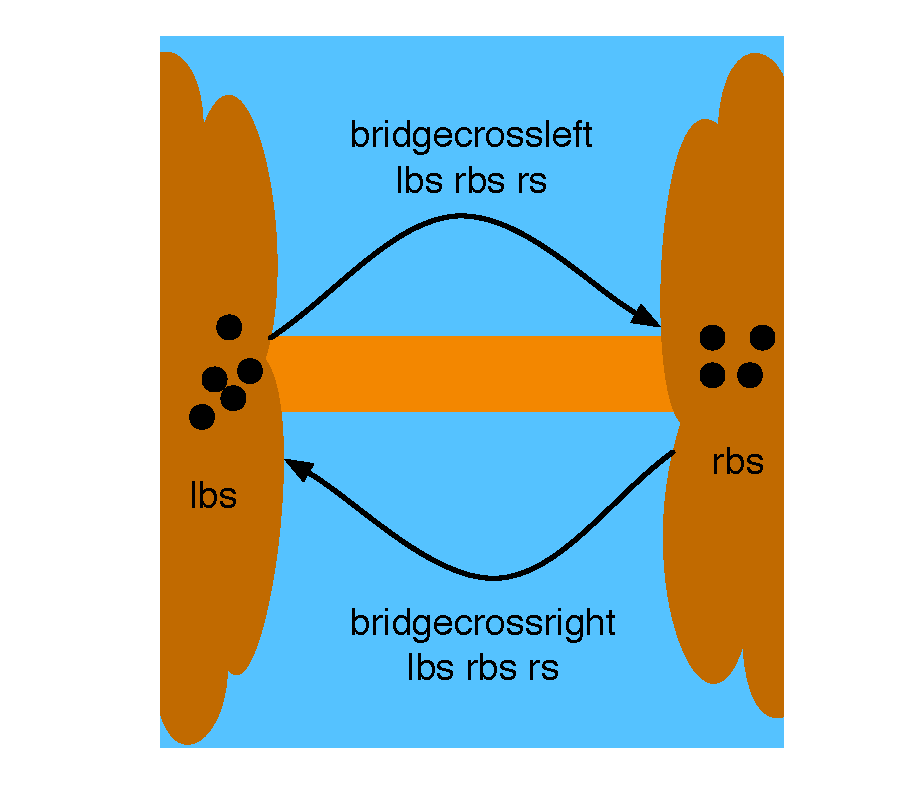
\includegraphics[width=2in]{fig.pdf}
\caption{Two mutually recursive functions \emph{bridgecrossleft} and \emph{bridgecrossright}.}
	\label{bridge_crossing_gen}
\end{marginfigure}

Calling \emph{bridgecross [1, 2, 3]} we get this result:

\begin{lstlisting}
[
 [(1,2),(1,1),(1,3)],
 [(1,2),(2,2),(2,3)],
 [(1,3),(1,1),(1,2)],
 [(1,3),(3,3),(3,2)],
 [(2,3),(2,2),(2,1)],
 [(2,3),(3,3),(3,1)]
]
\end{lstlisting}


\newpage

\lstinputlisting[language=Haskell, basicstyle=\small, frame=trBL, caption={Haskell code}]{bridge.hs}
